\chapter{Conclusiones y trabajos futuros} \label{cap:conclusiones}

En este ultimo capítulo se exponen las conclusiones del proyecto tras todo el proceso de implementación y la obtención de los resultados. Se plantearán también las posibles líneas de trabajo futuro.

\section{Conclusiones}

En química, hay una serie de reglas establecidas para las que la mayoría de moléculas convencionales se ajustan bien, por lo que los paquetes software se diseñaron en su momento siguiendo esas reglas. Pero existen también muchas excepciones y particularidades, macromoléculas, proteínas, o compuestos de coordinación y organometálicos que no siguen las normas convencionales de las valencias y tipos de enlaces propios de la química orgánica o inorgánica, de modo que no se obtienen los resultados esperados.

Tras realizar un análisis de cómo ciertas bases de datos almacenan moléculas organometálicas, comparando los SMILES canónicos que ofrecen y sus representaciones gráficas, es evidente una inconsistencia entre ellas. En la actualidad, cada software implementa los algoritmos de canonización con unas reglas u otras, obteniendo SMILES canónicos que no son canónicos universales. Realmente el problema que se tiene entre manos no son los algoritmos en sí, sino que todo el mundo utilice el mismo algoritmo de generación canónico, una tarea compleja que requiere el consenso de toda la comunidad investigadora y los organismos detrás de las bases de datos.


Se pretende por tanto con este trabajo, \textit{hacer una propuesta} con el objetivo de resolver los conflictos entre las distintas bases de datos, usando una nueva nomenclatura canónica para moléculas organometálicas y mejoras en su dibujado.
Se aspira que en algún momento los cambios planteados se agreguen al software oficial de OpenBabel, se desplieguen en un futuro release, y con el tiempo se extienda su uso y sea útil para los que utilizan esta herramienta. La química es una ciencia que abarca muchas áreas y la creación de nuevas funcionalidades en la química computacional sigue en continuo avance. Con el desarrollo de este TFG en concreto se hace una contribución para el campo de la organometálica, y dada la naturaleza open-source de la herramienta utilizada, esperamos que la comunidad investigadora y de desarrolladores lleve estos cambios a otros paquetes software propiciando nuevos avances.


En general, consideramos que se han alcanzado resultados satisfactorios tanto para la nomenclatura canónica como para la modificación del sistema de representación aplicado al conjunto de datos con el que se ha trabajado. Si bien se utiliza un conjunto de datos relativamente pequeño, este se ajusta bien al alcance de un proyecto de estas características. Además ha sido proporcionado por los expertos de manera que contiene moléculas de interés para ellos. En base a sus recomendaciones también he centrado mis esfuerzos en mejorar el tipo de enlaces típicos en organometálica (las estructuras Cp),
cumpliendo así con todos los objetivos del proyecto.




\section{Trabajos futuros}

Tras todo el tiempo dedicado al proyecto y viendo los puntos débiles en esta área, creo que existen varios puntos clave a tratar en un futuro. 

\begin{itemize}
    \item Extender la aplicación del estudio y realizar pruebas con un conjunto de moléculas considerablemente mayor, adaptando poco a poco el sistema de dibujado para que se ajuste a las excepciones que se vayan presentando.
    
    \item Incluir más información sobre estereoquímica para las moléculas. Aún cuando la especificación de OpenSMILES incluye reglas para especificar la geometría alrededor de un átomo, ya sea tetraédrica, cuadrada plana, bipiramidal trigonal u octaédrica; debido a las complejidad de las tres últimas, en las bases de datos y en todos los SMILES que se pueden encontrar públicos en Internet, solamente se añade información de estereoquímica básica mediante los símbolos `$@$' y `$@@$' que indican centros tetraédricos \cite{opensmiles, crystallography_quiros}. Incluso la tetraédrica no se incluye en muchos SMILES. Por ejemplo, según los expertos (Anexo \ref{apend:expertos_dibujos}) hay varias moléculas con geometrías tetraédricas dentro del dataset, pero los SMILES de las bases de datos no lo expresan. Se podría investigar más este tema y estudiar su inclusión en la nomenclatura SMILES.
    
    A priori puede no parecer muy importante que se dibuje una línea plana o con cierta geometría, pero en ciertas áreas de la medicina y la bioquímica que trabajan con enzimas y pequeñas proteínas, un determinado fármaco según su geometría o isomería puede tener efectos completamente distintos.
    
    \item Conseguir la rotación de las estructuras Cp para ajustarse adecuadamente a casuísticas como los de la siguiente figura. 
    
        \begin{figure}[h!]
            \centering
            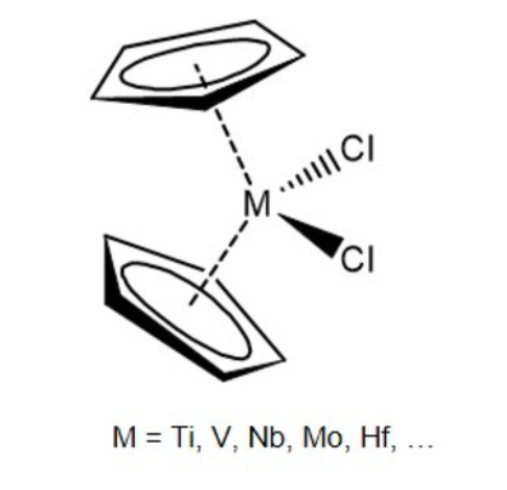
\includegraphics[scale=0.35]{imagenes/bent_metallocene.png}
            \caption{Metalocenos con disposición tetraédrica (en inglés, \textit{bent metallocenes}) usados por ejemplo en la investigación de fármacos anticancerígenos. Imagen extraída de \cite{bent_metallocenes}.}
            \label{fig:enter-label}
        \end{figure}
    
\end{itemize}
